\lettrine[lines=2,slope=0pt,nindent=4pt]{\textbf{I}}{n} this last part, the test cases correspond to two-phase flows at
local scale. Direct numerical simulations of such flows consist in
modeling two incompressible and immiscible fluids separated by a mobile
interface. The mass and impulsion balance equations hold for each
bulk phase with the viscosity and density of each fluid. The temperature
equation is neglected as well as phase change but the gravity is considered.
In such an approach, bubbles or drops are described individually with
their surface tension and the main difficulty is to follow accurately
interfaces that evolve in space and time. Several numerical methods
are dedicated to such interface tracking. They can be gathered into
two main families: ``diffuse interface method'' and ``sharp interface
method''. In \texttt{TrioCFD}, interfaces are tracked by ``Front-Tracking'',
a sharp interface method, for which the surface of separation between
both fluids is discretized by an additional lagrangian mesh. A re-meshing
is required during the calculation with a fine adjustment of numerical
parameters. In this part, the method is used for simulating problems
of \textbf{oscillating bubble} and \textbf{hanging drop}.\vspace*{3cm} \newline
\begin{center}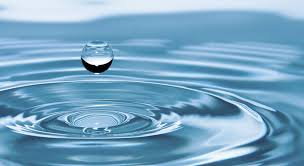
\includegraphics[width=12cm]{tools/goutte.png}\end{center}
